%!TEX root = ../thesis.tex
%*******************************************************************************
%****************************** Third Chapter **********************************
%*******************************************************************************
\chapter{Fraud Detection Pipeline}
\label{fraud_detection_pipeline}

\ifpdf
    \graphicspath{{Chapter3/Figs/Raster/}{Chapter3/Figs/PDF/}{Chapter3/Figs/}}
\else
    \graphicspath{{Chapter3/Figs/Vector/}{Chapter3/Figs/}}
\fi

\vspace*{\fill}
\thispagestyle{empty}
\epigraph{Standing on the shoulders of giants }{ --- Bernard of Chartres}
\thispagestyle{empty}

There are various research and studies on fraud detection problem and related issues,  including what algorithms should be used \citep{leonard1993detecting, bolton2001unsupervised, mahmoudi2015detecting}, how to prepare features \citep{bahnsen2016feature, whitrow2009transaction, fast2007relational}, \dots. In this section, we will review challenges in building the Fraud Detection System and its relevant questions. Based on that, we propose a Fraud Detection Pipeline which is not only simple, reliable but also easy to implement. Furthermore, we provide the readers many potential improvements for the pipeline.


\section{Imbalanced dataset}
\label{imbalanced_dataset}

One of the main problems of fraud detection is dataset imbalanced, i.e. the number of fraudulent transactions are a small fraction of the dataset \citep{juszczak2008off}. The imbalanced problem is of significant concern in the data mining and machine learning community because imbalanced datasets are common in many real-world domains. For instance, in the detection of fraudulent cases in telephone calls \citep{fawcett1997adaptive} and credit card transactions \citep{chan1999distributed}, the number of legitimate transactions heavily outnumbers the number of fraudulent transactions. Learning from imbalanced data sets is an important issue in supervised learning, with the credit card fraud detection problem, the imbalance is a big problem for the learning process. Let consider an example which consists only 1\% fraudulent transactions (minority class) and the remaining belongs to legitimate category (majority class), a lazy classification that predicts all of the transactions are legitimate transactions will has 99\% accuracy. This is a very high accuracy but we can not use this because it cannot detect any fraudulent transactions at all.

There are several methods that have been proposed to deal with the imbalanced problem and these could be separated into two levels: methods that operate at the data level and at the algorithmic level \citep{chawla2004special}. Algorithms at the algorithmic level are designed to deal with the minority class detection and at the data level, the rebalanced strategies are used as a pre-processing step to rebalance the dataset before any algorithm is applied.


\subsection*{Algorithmic level methods}
\label{algorithmic_level_methods}


At algorithmic level, these algorithms are modified or extended of existing classification algorithms for imbalanced tasks. Based on their styles we can separate these algorithms into two styles: imbalanced learning and cost-sensitive learning. In the first learning, the algorithms try to improve the accuracy of the minority class prediction, while the second learning tries to minimize the cost of wrong predictions.


\subsubsection*{Imbalance learning}
\label{imbalance_learning}

Decision tree, e.g. C4.5 \cite{quinlan2014c4}, use Information Gain as splitting criteria to maximize the number of predicted instances in each node, it makes the tree bias towards the majority class. Cieslak and Chawla \citep{cieslak2008learning} suggest splitting with Hellinger Distance (HD) which they show that HD is skew-insensitive and their proposed Hellinger Distance Decision Tree is of better performance compared to the standard C4.5. Other studies have also reported the negative effect of skewed class distributions not only in decision tree \citep{he2009learning, japkowicz2002class}, but also in Neural Network \citep{japkowicz2002class, visa2005issues}, k-Nearest Neighbor (kNN) \citep{kubat1997addressing, mani2003knn, batista2004study} and SVM \citep{yan2003predicting, wu2003class}.

In Machine Learning, with a great success of ensemble learning on several applications, many ensemble strategies have been proposed for imbalanced learning. Bagging \citep{breiman1996bagging} and Boosting \citep{freund1996experiments} are the most popular strategies which combine the imbalanced strategy with a classifier to aggregate classifiers \citep{liu2009exploratory, wang2009diversity, vilarino2005experiments, kang2006eus, liu2006boosting, wang2010boosting, chawla2003smoteboost, joshi2001evaluating, mease2007boosted}.


\subsubsection*{Cost-sensitive learning}
\label{cost_sensitive_learning}

In classification applications dealing with imbalanced datasets, the correct prediction of minority class is more important than the correct prediction of majority class, which causes several classifiers to fail when predicting minority class because they assume the cost of these classes are the same. In the credit card fraud problem, the cost of our true prediction is zero, but if we cannot detect a fraud transaction then its amount of money is our lost and if we predict a non-fraud is a fraud then the cost is an investigation fee need to correct this transaction (see table \ref{tab:simple_cost_matrix} for a simple cost matrix).


\begin{table}[h!]
  \centering
  \caption{A simple cost matrix for one transaction.}
  \label{tab:simple_cost_matrix}
  \begin{tabular}{|c|c|c|}
      \hline
    &Non-fraud&Fraud \\
    \hline
    Predict non-fraud&0&its amount of money \\ \hline
    Predict fraud&investigation fee&0 \\ \hline
  \end{tabular}
\end{table}


Classifiers in cost-sensitive learning use different costs for prediction of each class, these cost-based classifiers could handle wrong-prediction costs without sampling or modifying the dataset. For example in tree-based classifiers, cost-based splitting criteria are used to minimize costs \citep{ling2004decision}; or used in tree pruning\citep{bradford1998pruning}. An extension of cost-sensitive learning, Domingos proposed Metacost \citep{domingos1999metacost} framework that transforms non-cost-sensitive algorithm into a cost-sensitive algorithm. However, the cost for minority class is usually not available or difficult to compute, which makes the cost-sensitive algorithms are not popular \citep{maloof1997learning}.


\subsection*{Data level methods}
\label{data_level_methods}

Methods at data level are techniques that modifying an imbalanced dataset before any classifiers could be applied. In this section, we will introduce some popular techniques usually used to re-balance the distribution of the classes.


\subsubsection*{Sampling}
\label{sampling}

Several studies \citep{weiss2001effect, laurikkala2001improving, estabrooks2004multiple} have shown that balanced training set will give a better performance when using normal algorithms, and sampling methods are the most common techniques in data science to create a balanced training set. There are three popular sampling techniques, including undersampling, oversampling and SMOTE (see figure \ref{sampling_methods}); and some extension sampling techniques are based on these three techniques, e.g. Borderline-SMOTE \citep{han2005borderline}, ADASYN \citep{he2008adasyn}, \dots.

Undersampling \citep{drummond2003c4} is a method to decrease the size of the majority class by removing instances at random. The idea is that many instances of the majority class are redundant and the removal of these instances, thereby, makes its distribution change not too much. However, the risk of dropping redundant instances still exists since this process is unsupervised and we cannot control what instances will be dropped. Furthermore, a perfectly balanced dataset, which means the size of the minority class equals the size of the majority class, is not a good choice for undersampling \citep{dal2015calibrating}. In practice, this technique is often used because it is simple and speeds up our process.

Oversampling \citep{drummond2003c4} is an opposite method of undersampling that tries to increase the size of minority class at random. While duplicating the minority class, oversampling increases a risk of overfitting by biasing the classifier toward the minority class \citep{drummond2003c4}. Furthermore, this method does not add any new information for minority instances and it also slows down our learning phase.

SMOTE \citep{chawla2002smote} is a small extended version that combines both sampling techniques above, abnormal oversampling and normal undersampling. While oversamples the minority class by creating similar instances in a neighborhood area and also do undersampling the majority instances randomly, it could create clusters around each minority instance and helps classifiers build larger decision regions. SMOTE has shown to increase the accuracy of classifiers \citep{chawla2002smote}, a change of learning time depends on sampling ratio but it still has some drawbacks, e.g. new minority instances are created without considering its neighborhood so it increases the overlapping area between the classes. \citep{wang2004imbalanced}.


\begin{figure}[!ht]
\centering
\caption{Three common sampling methods \citep{dal2013racing}}
\label{sampling_methods}
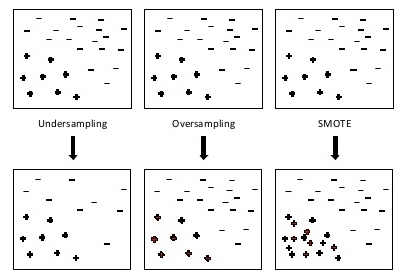
\includegraphics[]{Images/sampling_methods.jpg} 
\end{figure}


\subsubsection*{Cost-based}
\label{cost_based}

Cost-based methods is a kind of sampling technique that considers the misclassification cost which is assigned to each instance a different value. The above sampling techniques are random, with cost-based sampling methods, the weight of minority class is usually higher than the weight of majority class and then other sampling techniques could be used to rebalance the datasets.

Costing \citep{zadrozny2003cost} is a cost-based undersampling that draws instances with an acceptable probability greater than a pre-defined threshold. Klement et al. \citep{klement2009cost} proposed a more complicated and effective approach that combines cost-based random under-sampling and ensemble learning. The cost-based methods are promising when dealing with imbalanced datasets, however, the cost of misclassification for each class may be not easy to see in the real life as we have mentioned in the section above.
 

\subsubsection*{Distance-based}
\label{distance_based}

Distance-based methods are slightly different than cost-based methods, i.e. instead of considering the cost of misclassification. These methods consider a distance among instances in the imbalanced dataset to undersample or to remove a noise and borderline instances of each class. They need to compute the distance between instances so these methods are more costly than the above methods.

Tomek \citep{tomek1976two} proposed a method that removes instances from the majority class that is close to the minority region in order to have a better separation between two classes. His method is useful in noisy datasets or datasets with the overlapping problem, i.e. removing those instances can make the classifier toward misclassification \citep{suman2005methods}. There are several distance-based sampling studies, e.g. Condensed Nearest Neighbor \citep{hart1968condensed}, One Sided Selection \citep{kubat1997addressing}, Edited Nearest Neighbor \citep{wilson1972asymptotic} or Neighborhood Cleaning Rule \citep{laurikkala2001improving}.


\section{Algorithms}
\label{algorithms}

In the fraud detection problem, almost Machine Learning algorithms, including supervised learning \citep{chan1999distributed, kubat1997addressing, bhattacharyya2011data}, unsupervised learning \citep{tasoulis2006unsupervised, bolton2001unsupervised}, ..., have been proposed to detect fraudulent transactions. In this section, we will see which algorithms are used to solve the fraud detection problem.


\subsection*{Expert Systems}

In the very early 90s, the decision which decides a transaction is a fraud or not follows from rules and the rules are generated from the knowledge of human expert. Expert's rules are just simple IF-THEN rules and extremely manually since all of the rules based on the expert's knowledge and ability. By applying expert system, suspicious activity or transaction can be detected from deviations from normal spending patterns \cite{leonard1995development}. Kevin at el. proposed expert system model to detect fraud for alert financial institutions \cite{leonard1993detecting}. Nik presented a FUZZY system to detect credit card frauds in various payment channels, their model fuzzy expert system gives the abnormal degree which determines how the new transaction is fraudulent in comparison with user behavioral \cite{haratinik2012fuzzgy}.


\subsection*{Association Rules}

Association rules are an extended approach of Expert Systems in which we add a certainty factor for expert's rules. Usual measures for the certainty are proposed by Agrawal et al \cite{agrawal1993mining} for establishing an association rule’s fitness and the interest
are the confidence $Conf(A \Rightarrow C)$, the conditional probability $p(C \mid A)$, the support $Supp(A \Rightarrow C)$, and the joint probability $p(A \cup C)$, \dots.

There are few studies use association rules and its extension, e.g. fuzzy association rules \cite{sanchez2009association}. However, the expert's rules are still generated manually and it is the biggest disadvantage of those methods. In the current computing age, a complexity of the data is increasing fastly and we need to create rules or make fraud prediction automatically.


\subsection*{Neural Networks}

The neural networks are non-linear statistical data modeling tools that are inspired by the functionality of the human brain using a set of interconnected nodes \citep{yeh2009comparisons, ghosh1994credit}. Because of its strengths, neural networks are widely applied in various applications such as automobile insurance and corporate fraud. The literature describes that neural networks can be used as a financial fraud detection tool. The neural network fraud classification model employing endogenous financial data created from the learned behavior pattern can be applied to a test sample \citep{green1997assessing}. The neural networks can be used to predict the occurrence of corporate fraud at management level \citep{cerullo1999using}.

Researchers have explored the effectiveness of neural networks, decision trees and Bayesian belief networks in detecting fraudulent financial statements (FFS) and to identify factors associated with FFS \citep{kirkos2007data}. The study in \citep{fanning1998neural} revealed that input vector consisted of financial ratios and qualitative variables, was more effective when fraud detection model was developed using the neural network. The model was also compared with standard statistical methods like linear and quadratic discriminant analysis, as well as logistic regression methods \citep{fanning1998neural}.

The Bayesian belief network (BBN) is a graphical model that presents a probabilistic dependency using a directed acyclic graph (DAG), in which nodes represent random variables and missing edges encode conditional independencies between the variables \citep{kirkos2007data}. The Bayesian belief network is used in developing models for the credit card, automobile insurance, and corporate fraud detection. Bayesian belief network outperformed neural network and decision tree methods and achieved outstanding classification accuracy \citep{kirkos2007data}.


\subsection*{Logistic Regression (LR)}

Logistic Regression \cite{walker1967estimation, cox1958regression} is an important machine learning algorithm. The goal of LR is to model the probability of a target belong to each class. Logistic Regression is a simple and efficient approach that is a widely used technique in such problems \cite{hosmer2013applied}. There are many studies tried to use logit models to estimate fraudulent probability in the case of insurance frauds \cite{jin2005binary, artis2002detection} and other related areas like food stamp programs, and so forth \cite{bollinger1997modeling, hausman1998misclassification, poterba1995unemployment}.


\subsection*{Decision Tree}

A Decision Tree is a decision support tool that uses a tree-like graph to find a prediction rule from the labeled dataset. In our fraud detection case, this means that it could generate expert-rules IF-THEN automatically. The Decision Tree has many advantages, e.g. simple to understand and interpret, important insights can be generated automatically like experts, \dots and it has found several applications in fraud detection \citep{csahin2011detecting, sahin2013cost, bahnsen2015example, lee2006mining}.


\subsection*{Random Forest}

Random Forest \citep{breiman2001random} is an ensemble of Decision Trees, where each tree is trained on a different bootstrap sample of the original training set and uses a random subset of all the features available. The forest of Decision Trees that are very different from each other, this diversity is a key factor for variance reduction in order to overcome the disadvantage of Decision Tree \citep{krogh1995neural}.

Several studies have shown that it achieves the best results among different classifiers \citep{dal2014learned, dal2015credit, van2015apate, whitrow2009transaction, bhattacharyya2011data, bahnsen2013cost} when using Random Forest. Pozzolo et al. \citep{dal2013racing} have shown that the Random Forest combined with undersampling or SMOTE are often the best choice. In our case, we refer undersampling over SMOTE since our data is usually huge. We propose using Random Forest with undersampling for many reasons, e.g. powerful, fast, simple to interpret, \dots.


\section{Sample Selection Bias}
\label{sample_selection_bias}

A standard assumption, not only in Data Science but also in Statistics, is stationary, i.e. the training set and testing set have the same distribution, since these sets come from one generating source. In a non-stationary environment, there is a distributional mismatch between the training set and testing set and classifiers are fitted using the training set could not use the testing set to check its accuracy.

This situation could occur when we modify the original dataset, e.g. under-sampling, and a newly created training set doesn't represent well for the whole dataset. We called this a Sample Selection Bias (SSB), which also happens in the collecting data step when we do not or could not collect data that present the population distribution. For example, when predicting a new customer that could pay a loan (and its interest) at the end of this month and we give a try with a current data of a bank, however the bank only records old customers that repay and they directly refuse a new bad customer without recorded information.

Let $s$ is a random variable which takes either 1 (sampled) or 0 (not sampled). Using Bayes formula we could re-write the $P(x,y)$ as:


\begin{equation}
P(x, y) = \dfrac{ P(x, y|s = 1)P(s = 1) }{ P(s = 1|x, y) } = \dfrac{ P(s = 1) }{ P(s = 1|x, y) } P(x, y|s = 1)
\end{equation}


As initially proposed by Zadrozny \citep{zadrozny2004learning} there were four types of conditional dependencies:

\begin{itemize}
\item No \textit{sample selection bias} or $P(s = 1|x, y) = P(s = 1)$. In other words, the selection process is independent from both feature vector $x$ and class label $y$,
\item \textit{Feature bias} or $P(s = 1|x, y) = P(s = 1|x)$. The selection process is conditionally independent from $y$ given $x$ . It is important to understand that feature bias does not imply $s = 1$ is completely independent from $y$,
\item \textit{Class bias} or $P(s = 1|x, y) = P(s = 1|y)$. The selection process is conditionally independent from $x$ given $y$. Similarly, it does not imply that $s = 1$ is completely independent from $x$,
\item \textit{Complete bias} or $P(s = 1|x, y)$. The selection process is dependent on both $x$ and $y$.
\end{itemize}


There are many research studies relate to the SSB \citep{elkan2001foundations, zadrozny2003cost, zadrozny2001learning, zadrozny2004learning, fan2005improved, dudik2006correcting}. One approach for this problem is \textit{important sampling} that assign a weight to each data point \citep{zadrozny2003cost, zadrozny2004learning, fan2005improved}. The $P(x,y)$ re-writes in term of $P(x, y|s = 1)$ then we could do sampling with the weight $\dfrac{ P(s = 1) }{ P(s = 1|x, y) }$, but it is not an easy task due to estimating $P(s = 1|x, y)$ is not straightforward. Instead of trying to find what sample well represents the dataset, another simpler approach to handle SSB is using ensemble learning to combine results from multiple samples or from multiple classifiers \citep{fan2007sample}.

In the previous section, we preferred to use Random Forest with the undersampling method and this approach could lead to the Sample Selection Bias problem. In order to avoid it, we propose using ensemble method that will combine multiple Random Forests classifiers. Splitting the dataset into multiple subsets by applying the undersampling technique, each subset will be used as the training set of Random Forest. A final prediction could be mean or mode of these classifiers and it makes the final result more stable because we use all of the available data. We will give more details of this method in the following chapter.


\section{Feature Engineering}
\label{feature_engineering}

One of the most important steps in Machine learning is Feature Engineering which we will pre-process features in the dataset to improve the accuracy of a algorithm. The Feature Engineering usually consist: impute missing values, detect outliers, extract new useful features, \dots. A set of raw attributes in many credit card datasets is quite similar because the data collected from a transaction must comply with international financial reporting standards (American Institute of CPAs, 2011) \citep{aicpa}. Typical attributes in one credit card dataset are summarized in table \ref{tab:typical_raw_attributes}, these attributes could be grouped into four levels:

\begin{itemize}
\item Transaction level: these features typically are the raw attributes of the transaction which are collected in real time,
\item Card level: spending behavior of a card could be computed by aggregating information from transactions made in last given hours of a card,
\item User level: spending behavior of the customer, in some cases one user has only one card and these levels are the same,
\item Network level: users in our system are not isolated, they are connected and share the behavior, we will discuss this level in the next section.
\end{itemize}


\begin{table}
\centering
\footnotesize
\caption{List of typical raw attributes in a transaction dataset}
\label{tab:typical_raw_attributes}
\begin{center}
 \begin{tabular}{||c | c||} 
 \hline
 Attribute name & Description \\ [0.5ex] 
 \hline\hline
 Transaction ID & Transaction identification number \\ 
 \hline
 Time & Date and time of the transaction \\
 \hline
 Account number & Identification number of the customer \\
 \hline
 Card number & Identification of the credit card \\
 \hline
 Transaction type & ie. Internet, ATM, POS, ... \\
 \hline
Entry mode & ie. Chip and pin, magnetic stripe, ... \\
\hline
Amount & Amount of the transaction in Euros \\
\hline
Merchant code & Identification of the merchant type \\
\hline
Merchant group & Merchant group identification \\
\hline
Country & Country of transaction \\
\hline
Country 2 & Country of residence \\
\hline
Type of card & ie. Visa debit, Mastercard, American Express... \\
\hline
Gender & Gender of the card holder \\
\hline
Age & Card holder age \\
\hline
Bank Issuer & bank of the card \\
 [1ex] 
 \hline
\end{tabular}
\end{center}
\end{table}


There are many studies use only raw transactional features, e.g. time, amount, \dots and don't take into account the spending behavior of the customer, which is expected to help discover fraud patterns \citep{lebbe2008artificial}. Standard feature augmentation consists of computing variables such as average spending amount of the cardholder in the last week or last month, number of transactions in the same shop, number of daily transactions, \dots \citep{dal2014learned, krivko2010hybrid, whitrow2009transaction, bhattacharyya2011data, jha2012employing}.

Whitrow et al. proposed a transaction aggregation strategy in order to aggregate customer behavior \citep{whitrow2009transaction}. The computation of the aggregated features consists in grouping the transactions made during the last given number of hours by each categorical features, e.g. card id, user id, transaction type, merchant group, country or other, followed by calculating the average/total/\dots amount spent on those transactions. This methodology has been used by a number of studies \citep{bhattacharyya2011data, bahnsen2013cost, dal2014learned, jha2012employing, sahin2013cost, tasoulis2008mining, weston2008plastic}. Whitrow et al. \citep{weston2008plastic} proposed a fixed time frame to be 24, 60 or 168h, Bahnsen et al. \cite{bahnsen2016feature} extended time frames to: 1, 3, 6, 12, 18, 24, 72 and 168h.

The process of aggregating features consists in selecting those transactions that were made in the previous $t_p$ hours, for each transaction $i$ in the dataset $S$:


\begin{equation}
S_{agg} = T_{agg} (S, i, t_p) \\
\quad = \lbrace x_j^{amount} \mid ( x_j^{feature} = x_i^{feature} ) \wedge (H(x_i^{time}, x_j^{time}) < t_p) \rbrace
\end{equation}


where:

$T$: function creates a subset of S associated with a transaction $i$ with respect to the time frame $t_p$,

$x_i^{amount}$: the amount of transaction $i$,

$x_i^{feature}$: the categorical feature of transaction $i$ which is used to group the transactions,

$x_i^{time}$: the time of transaction $i$,

$H(t_1, t_2)$: number of hours between the times $t_1$ and $t_2$.

After that, we can compute a customer behavior in last given hours, for example, an average amount of this time frame:


\begin{equation}
x_i^{average\_amount} = \dfrac{1}{N} \sum_{x^{amount} \in S_{agg}} x^{amount}
\end{equation}


with:

$x_i^{average\_amount}$: a new feature computed from subset $S_{agg}$ by function average,

$N$: number of transactions in subset $S_{agg}$.

These new useful features above for capturing customer spending patterns, Bahnsen et al. \cite{bahnsen2016feature} are also interested in analyzing the time of a transaction. The logic behind this is a customer is expected to make transactions at similar hours. However dealing with the time of the transaction is not the same as dealing with the above features since the time in a day is the circle, therefore it is easy to make the mistake of using the arithmetic mean of transactions' time. They have proposed to overcome this limitation by modeling the time of the transaction as a periodic variable, in particular using the von Mises distribution \citep{fisher1995statistical}.

Recently Wedge et al. \citep{wedge2017solving} tried applying automated feature engineering with some simple functions to reduce the time cost of this time-consuming feature engineering step, they claimed that a number of false positives dropped by 54\% compared to their previous approach. In summary, the feature pre-processing is important and some above methods are simple, easy to compute and run in real time. At least, the fraud detection system should have some simple aggregations, e.g. average, for some periods, e.g. 24h.


\section{Measurement}
\label{measurement}

The most common measure for classification tasks is accuracy; however, in the imbalanced dataset it is a misleading assessment measure, as well as some other measures e.g. MME, BER, TPR and TNR, \dots. There are some measures could handle this problem, e.g. AUC, F-measure,\dots and a well-accepted measure for imbalanced classification is the Area Under the ROC Curve (AUC) \citep{chawla2009data}. AUC shows that how much the ROC curve is close to the perfect classification; however, Hand \citep{hand2009measuring} considers the standard calculation of the AUC as inappropriate because it making an average of different misclassification costs for classes. F-measure is more accurate in the sense that it is a function of a classifier and its threshold setting, i.e. it considers both the precision and the recall of the test to compute the score. The traditional F-measure or balanced $F_1$ score is the harmonic mean of precision and recall.

In many Fraud Detection System \citep{sahin2013cost, mahmoudi2015detecting, bahnsen2015example}, cost-based measures are defined to quantify the monetary loss due to fraud \citep{bahnsen2013cost} by computes average cost-matrix which is similar to the confusion matrix. Elkan \citep{elkan2001foundations} states that it is safer to assess the cost-sensitive problem in terms of benefit (inverse of cost) because there is the risk of applying different baselines when using a cost-matrix to measure overall cost. Dealing with this issue, normalized cost or savings \citep{bahnsen2015example} are used to judge the performance w.r.t. the maximum loss.

In the cost matrix, the cost of a missed fraud is often assumed to be equal to the transaction amount \citep{elkan2001foundations, bahnsen2013cost}, because it has to be refunded to a customer. Cost of false alert is considered to be equivalent to the cost of a phone call because our investigators have to make the phone call to the card-holder to verify a transaction whether it is a fraud or not. Furthermore, there are many intangible costs, e.g. reputation cost of a company, maintenance cost of the investigator's department, \dots. For all of these reasons, define a good cost measure is not easy in credit card fraud detection and there is no agreement on which is an appropriate way to measure the cost of frauds.

In a scenario with limited resources, e.g. there are only a few investigators, they can't check all alert transactions which are marked as fraudulent from the detection system. They have to put their effort into investigating transactions with those highest risk of fraud, in other words the detection system has to give each transaction its posterior fraud probability. With this requirement, the measure must contain the probability part in order to measures how good the system gives the high score to fraud transaction and reverse.

In summary, define a good measure to analyze the accuracy of the system is not easy, not only in our case but also in many other domains of Machine learning. Similar with the imbalanced problem, the cost-based measures seem very promising and we also need to know all of the cost for each instance. The $F-1$ score is better than all of the others, it is easy to compute and suitable for the imbalance problem, and we thereby will use the $F-1$ measure to evaluate our fraud detection pipeline.


\section{Fraud Network}
\label{fraud_network}

In the very early age of the computer, experts have noticed that a fraudulent account is often connected to another fraudster. This is true in many domains, for example in the telecommunication domain, therefore analyzing the links in the data could discover fraud networks and improve the accuracy of the system \citep{fast2007relational}.

The network not only could increase the true positives of our system, but also decrease the false positives. For example, consider the following legal scenario: a husband and his wife traveling to another country, the first transaction of the husband could create a fraud alert then the next transaction of his wife from the same city should be legal with or without confirmation of the first one.

Despite these advantages, aggregating fraud network-level features is not easy and recently had been taken with more consideration. Van Vlasselaer et al. have proposed APATE \citep{van2015apate}, a framework for credit card fraud detection that allows including network information as additional features describing a transaction. In the next year after APATE, they also proposed GOTCHA! \citep{van2016gotcha}, a novel approach which can improve the accuracy of traditional fraud detection tools in a social security context, this approach uses a time-weighted network and features extracted from a bipartite graph. They show that network-level features are able to improve significantly the performance of a standard supervised algorithm.

In summary, finding the network in the dataset is a complicated task and it's not the best choice for the first version of the fraud detection system.


\section{Concept Drift}
\label{concept_drift}

As mentioned in section \ref{sample_selection_bias}, the non-stationary environment could occur when we modify the dataset. In case a data generating source changes itself over time in an unforeseen manner, it is known as Concept Drift \citep{gama2014survey} or Dataset Shift \citep{quionero2009dataset}. With Bayes rule, we have a joint distribution of a sample $(x, y)$ is:


\begin{equation}
P(x, y) = P(y|x)P(x) = P(x|y)P(y)
\end{equation}


In classification tasks, we usually want to estimate the probability $P(y|x)$, from the above formula, we have:


\begin{equation}
P(y|x) = \frac{P(x|y)P(y)}{P(x)}
\end{equation}


From this Bayes formula, the change of data distribution at time $t$ and $t + 1$ could come from several sources\citep{kelly1999impact}:

\begin{itemize}
\item $P(y|x)$: a change occurs with a class boundary $( P_t(y|x) \neq P_{t+1}(y|x) )$, this makes any classifiers which are well designed will be biased,
\item $P(x|y)$: this change $( P_t(x|y) \neq P_{t+1}(x|y) )$ is a internal change within a class which is observed in an inside class but the class boundary isn't affected, also known as Covariate Shift \citep{moreno2012unifying},
\item $P(y)$: change in prior probability $( P_t(y) \neq P_{t+1}(y) )$, it makes a good design classifier become less reliable,
\item or combination of these three parts.
\end{itemize}

There is no $P(x)$ in the list because the change in $P(x)$ does not affect $y$ so we could ignore it \citep{hoens2012learning}.  In general, it is hard to say where the change comes from since we only see the generated data and we do not know or cannot control the data generating process. Learning in the non-stationary environment make us have to update models frequently to capture up-to-date patterns and also remove irrelevant patterns.

In fraud detection problem, we saw that fraudsters always try to create new fraudulent strategies to bypass our detection system, and new fraudsters also give a try with old strategies. Therefore, patterns in our system are learned from the past data may re-occur in the future then the removing process makes us losing the accuracy, this problem is known as the stability-plasticity dilemma \citep{grossberg1988nonlinear}.

In summary, dealing with Concept Drift problem, our fraud detection system has to update frequently to capture new fraudulent patterns as soon as possible, e.g. a bank has up-to-date labels at night then they could update their system daily.


\section{Delayed True Labels}
\label{delayed_true_labels}

Most of the supervised learning algorithms are based on the assumption that labels of the dataset are correct; however, in the real world environment it could be not true. In our case, the fraud detection problem, after the system generates alerts then with a limited number of investigators, only a restricted quantity of alerts could be checked. It means a small set of labeled transactions returned as \textit{feedback} and makes the unrealistic assumption that all transactions are correctly labeled by a supervisor.

Furthermore, non-alerted transactions are a large set of unsupervised instances that could be either fraudulent or genuine but we only know the actual label of them after customers have possibly reported unauthorized transactions and maybe available several days later. And the customers have different habits, e.g. rarely check a transcript of credit card given by the bank, which makes our dataset non-accurate and hard to modeling the fraudulent patterns.

In fraud detection problem, a company, e.g. a bank, usually has all latest up-to-date labels of transactions at night, and other companies could have after a longer time. It means that the system has to be updated frequently, i.e. as soon as possible after receives accurate labels. And the system which is never updated will lose their accuracy over the time.

Pozzolo et al. \citep{dal2015credit} claimed that the accurate up-to-date labels are very important and they proposed a learning strategy to deal with the feedback. Their method used both feedbacks $F_t$ and delayed supervised instances $D_{t-\delta}$:

\begin{itemize}
\item  a sliding window classifier $W_t$: daily updated classifier over the supervised samples received in the last $\delta$ + M days, i.e. $ \lbrace F_t, \dots, F_{t - (\delta - 1)}, D_{t-\delta}, \dots, D_{t- (\delta + M -1)} \rbrace $,
\item an ensemble of classifiers $\lbrace \mathcal{M}_1, \mathcal{M}_2, \dots, \mathcal{M}_M, \mathcal{F} \rbrace$ where $\mathcal{M}_i$ is trained on $D_{t - ( \delta + i - 1)}$ and $F_t$ is trained on all the feedbacks of the last $\delta$ days $\lbrace F_t, \dots, F_{t - (\delta - 1)} \rbrace$.
\end{itemize}

Their solutions used two basic approaches for handling concept drift that can be further improved by adopting dynamic sliding windows or adaptive ensemble sizes \citep{fan2004systematic}. In summary, to keep the accuracy of the system, we need to update all of the classifiers as soon as the data available, and usually it is a daily update.


\section{Performance}
\label{performance}

Particularly in fraud detection problem, we are dealing with a huge credit card transaction dataset. As we see in the sections above, many approaches are used to detect fraud transactions, many of them have shown that they have a good result with their approach, however, most of them could not be used in production because they did not consider their running time. For instance, in the age of Neural Network there are many studies try to use Neural Network models to detect fraud, but this approach runs the training process very slowly. 

In the age of Big Data, there are some frameworks for distributed computing system and the most common one currently used in many biggest system around the world is Spark \cite{zaharia2010spark}. Spark is an open-source cluster-computing framework, originally developed at the University of California, Berkeley's AMPLab. With Spark framework, we could distribute the computation for each transaction into one node in our cluster, and the cluster is easy to scale up.

Spark also supports Machine learning algorithms via its MLlib library \cite{meng2016mllib}. However, with the current version of Spark (2.2.0 \cite{spark220}), there are not many algorithms supported, which means that for those companies they have only a few options to build the detection system. Fortunately, some of the most common algorithms are supported, e.g. Linear Model, Decision Tree or Random Forest, \dots.


\section{Fraud Detection Pipeline}

We have discussed the challenges of building the Fraud Detection System and found out several possible ways to resolve them. Based on that, in this section, we analyze and propose a Fraud Detection Pipeline, which is not only easy to implement but also has a reliable result.


\subsection*{Imbalanced dataset and Algorithm}

The imbalance problem and algorithms in the fraud detection problem could be grouped into two groups based on our point of view:


\begin{itemize}
\item Theoretical perspective: apply Data Science and Data Mining to obtain a \textit{good} result like other applications,
\item Financial perspective: this task is a problem in financial institutions and they want to minimize their losing money.
\end{itemize}


However the detail of losing money is usually not published since it is sensitive data, therefore those cost-based methods are out of the scope of this report. Among the rest approaches, Pozzolo et al. \citep{dal2013racing} have shown that the Random Forest combined with undersampling or SMOTE often has the best result. In our case, we prefer undersampling over SMOTE because it could manage the huge dataset. Usage details of the undersampling and Random Forest algorithm are provided later.


\subsection*{Sample Selection Bias}

A chosen sampling technique, undersampling, leads to the Sample Selection Bias problem and in order to avoid it, we propose to use an ensemble method that combines results from multiple samples \citep{fan2007sample}. The dataset will be split into multiple dis-joint samples, each of which is used to train a Random Forest classifier then the final prediction could be the mean or the mode value of these classifiers (see figure \ref{img:single_rf}). This approach is also useful for the imbalance problem above and reduces training times of the Random Forest classifiers.


\begin{figure}
\centering
\caption{Building single model by combining multiple Random Forest classifiers (RF)}
\label{img:single_rf}
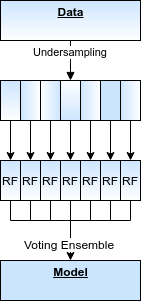
\includegraphics[scale=0.7]{Images/FDS_single_RF.png}
\end{figure}


\subsection*{Feature Engineering and Fraud Network}

Feature Engineering is one of the most important steps in Data Science and usually is difficult, time-consuming, and requires expert knowledge. We don't discuss in a detail this step, but in summary features after this step could be grouped into four levels:


\begin{itemize}
\item Transaction level: typically is the raw attributes of a transaction, which are available in real-time,
\item Card level: this level describes a spending behavior of a credit card, which is computed by aggregating the features from its previous transactions,
\item User level: usually same as card level if one user has only one card, it describes the spending behavior of a customer and a computing method is the same as card level,
\item Network level: detect Fraud Network in our system could improve the accuracy significantly but it is a complicated task, therefore we skip this level in our pipeline.
\end{itemize}


We propose to aggregate features which describe customer's behavior (user level and/or card level) consisting grouping transactions made during a last given number of hours by each categorical features, e.g. card id, user id, transaction type, \dots; followed by calculating some simple functions, e.g. average, amount spent on those transactions. The time frames could be 1, 3, 6, 12, 18, 24, 72, 168 hours and more. The detailed formulas are in section \ref{feature_engineering}.


\subsection*{Measurement}

Some common measures could not be used to evaluate the Fraud Detection System due to the imbalance problem. From the theoretical perspective, the simplest and suitable measure to deal with this is F1-score. Or inside a financial company, with all cost information on each transaction, we could use cost-based measures for those cost-based methods. In this thesis, we only use F1-score for its simplicity.


\subsection*{Concept Drift}

The data, which is fraudulent patterns and customer's behavior, always change over time. Dealing with this Concept Drift problem, all classifiers in our detection system have to update frequently to capture new patterns as soon as possible. We assume that we could update the system daily or at least every time frame, which is possible with a small dataset, and in the remaining of this chapter we will update all models at all time frames.


\subsection*{Performance}

As we have described in section \ref{performance} that to bring this Fraud Detection Pipeline into production, we have to consider its performance. And fortunately for us, the distributed computing framework Spark could handle our requirements, e.g. distribute our computation or run Machine Learning algorithms parallel, \dots. Therefore we propose to use this framework in both the development and the production phase.


\subsection*{Fraud Detection Pipeline}

With the Fraud Detection Pipeline architecture, we propose to build several models on different time frames for multiple purposes, such as:


\begin{itemize}
\item short-term model: using small latest data, e.g. one time frame data, to captures newest fraudulent strategies. In real life, it could be the last day or the last week data,
\item intermediate-term model: using more data than the above, i.e. longer period than short-term, e.g. two time frame data, to capture not only newest but also older fraudulent strategies. In real life, it could be the last month or last year data,
\item long-term model: similar with the above models but using more or all of the available data, e.g. three time frame data, to keep all possible fraudulent strategies in our data.
\end{itemize}


\begin{figure}
\centering
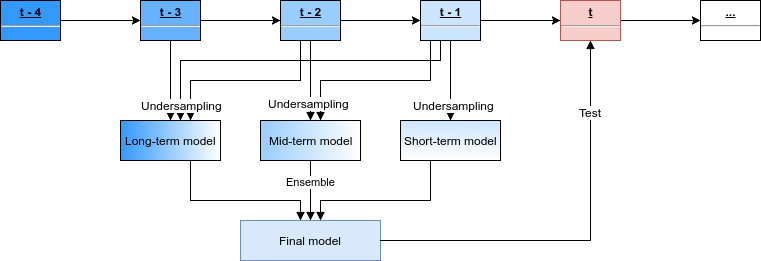
\includegraphics[width=\textwidth]{Images/FDS_diagram.png}
\caption{Recommended Fraud Detection Pipeline}
\label{img:fraud_detection_pipeline}
\end{figure}


The pipeline is summarized in figure \ref{img:fraud_detection_pipeline} and the detail of each model have been described above (see figure \ref{img:single_rf}). The size of the data and its training time increase from short-term to long-term model to accumulate fraudulent patterns. The long-term model needs a long time to prepare its new version and could be not available for the next day data, but with the fastest model, we could detect new fraudulent patterns while the new long-term model is training. This architecture could reduce workload for the slowest model and makes sure the system is always prepared for any possible situation.


\section{Upgrade the Fraud Detection Pipeline}

Since our proposed Fraud Detection Pipeline is a simple approach, there are several things could be done to improve the system and here we summarize some of the most potential improvements that will upgrade the current system easily:

\begin{itemize}
\item Imbalanced dataset: there are two main ideas to resolve this problem, one is the sampling methods and the other is cost-based methods. Our pipeline using the simpler way that does not need to know about the cost but it is very promising for the business view. We suggest trying to use the cost-based methods to have an overview of loss or saving money while using the system,
\item Algorithm: the supervised Random Forest algorithm had chosen as the main classifiers in the pipeline. We suggest expanding the models in the pipeline that could use more data or use other Machine Learning algorithms, e.g. the unsupervised learning to detect anomaly transactions or use stronger algorithms like Neural Networks, then finally combine all of classifiers to make the final prediction,
\item Feature Engineering: there are some profiling methods to capture customer's behaviors as we have described in section \ref{feature_engineering}. While the original attributes in the credit card dataset is limited, these aggregated features are very useful for the system and we strongly propose to apply all of these methods as the simplest way to upgrade the pipeline,
\item Measurement: the F1 score is the most suitable choice for the imbalance problem, therefore we do not need to change the metric. However, if we have the cost of each transaction, with or without the cost-based methods for both imbalance problem and algorithms, we suggest having one cost-based measure to see how much the money the system could save for a company,
\item Fraud Network: finding a network of fraudulent transactions in the data could improve the accuracy significantly. However, this task is not easy and requires complex researches so we suggest the readers only give a try with it after resolving all of the other things,
\item Delayed True Labels: the delayed labels are very important since it is the up-to-date and accurate labels. We suggest extending the Algorithms section above with one model using this data and with wrong predictions of our models, it could not only predicts the true delayed labels but also explains why our prediction fails,
\item Performance: the FDS usually need to process a very large number of transactions. While the distributed-computing Spark framework could handle it and also fits with other industry's requirements, therefore we do not have any reason to find an alternative solution and we suggest using the Spark framework in our system.
\end{itemize}


\section{Experiments and results}

Credit card transactions are very sensitive data, therefore there are only a few public datasets on the internet, some of them are very obsolete and do not have too many transactions. Fortunately there is one new and large transaction dataset which is published by Pozzolo et al. \citep{dal2015calibrating} in 2016, this dataset contains transactions made in September 2013 by European cardholders. It presents transactions that occurred in two days, where we have 492 frauds out of 284,807 transactions. This dataset is highly unbalanced, the positive class (fraudulent transactions) is 0.172\% of all transactions, i.e. imbalance ratio is 577.

The dataset contains only numerical input variables which are the result of a PCA transformation. Unfortunately, due to confidentiality issues, they cannot provide the original features and more background information about the data. Features \textit{V1}, \textit{V2},\dots, \textit{V28} are the principal components obtained with PCA; the only features which have not been transformed with PCA are \textit{Time} and \textit{Amount}. The feature \textit{Time} contains the seconds elapsed between each transaction and the first transaction in the dataset, the feature \textit{Amount} is the transaction's amount. Column \textit{Class} is the response variable and it takes value 1 in case of fraud and 0 otherwise.

In this thesis, we use this dataset to test the proposed Fraud Detection Pipeline and also for other studies below. Splitting this dataset into 48 time frames, we use the first 24 time frames for a training phase and the rest for the testing phase. Testing with three window lengths, short-term, intermediate-term and long-term periods are 1,2 and 3 time frames respectively. We run a stratified 5-fold cross-validation then compute the metric $F_1$ score as an average of five folds. This study runs on one single machine with 24 cores CPU and 128 gigabytes memory. The result is in figure \ref{img:fdp_summary} and a detail is in table \ref{tbl:fdp_summary}. 

In the result, the short-term model often fails with zero $F_1$ score if it does not re-train anymore and compare with daily update, the model will be improved significantly (81\%). Only the long-term model with the daily update has a bit lower accuracy than the never update model (1\%). As we forecast above, the more data we use in the longer term model the more accuracy we have, i.e. the long-term model with $F_1$ score is 22\% higher than the short-term model. In general, the daily update mechanism usually better in both average and standard deviation of $F_1$ scores over 5-fold cross-validation.


\begin{figure}
\centering
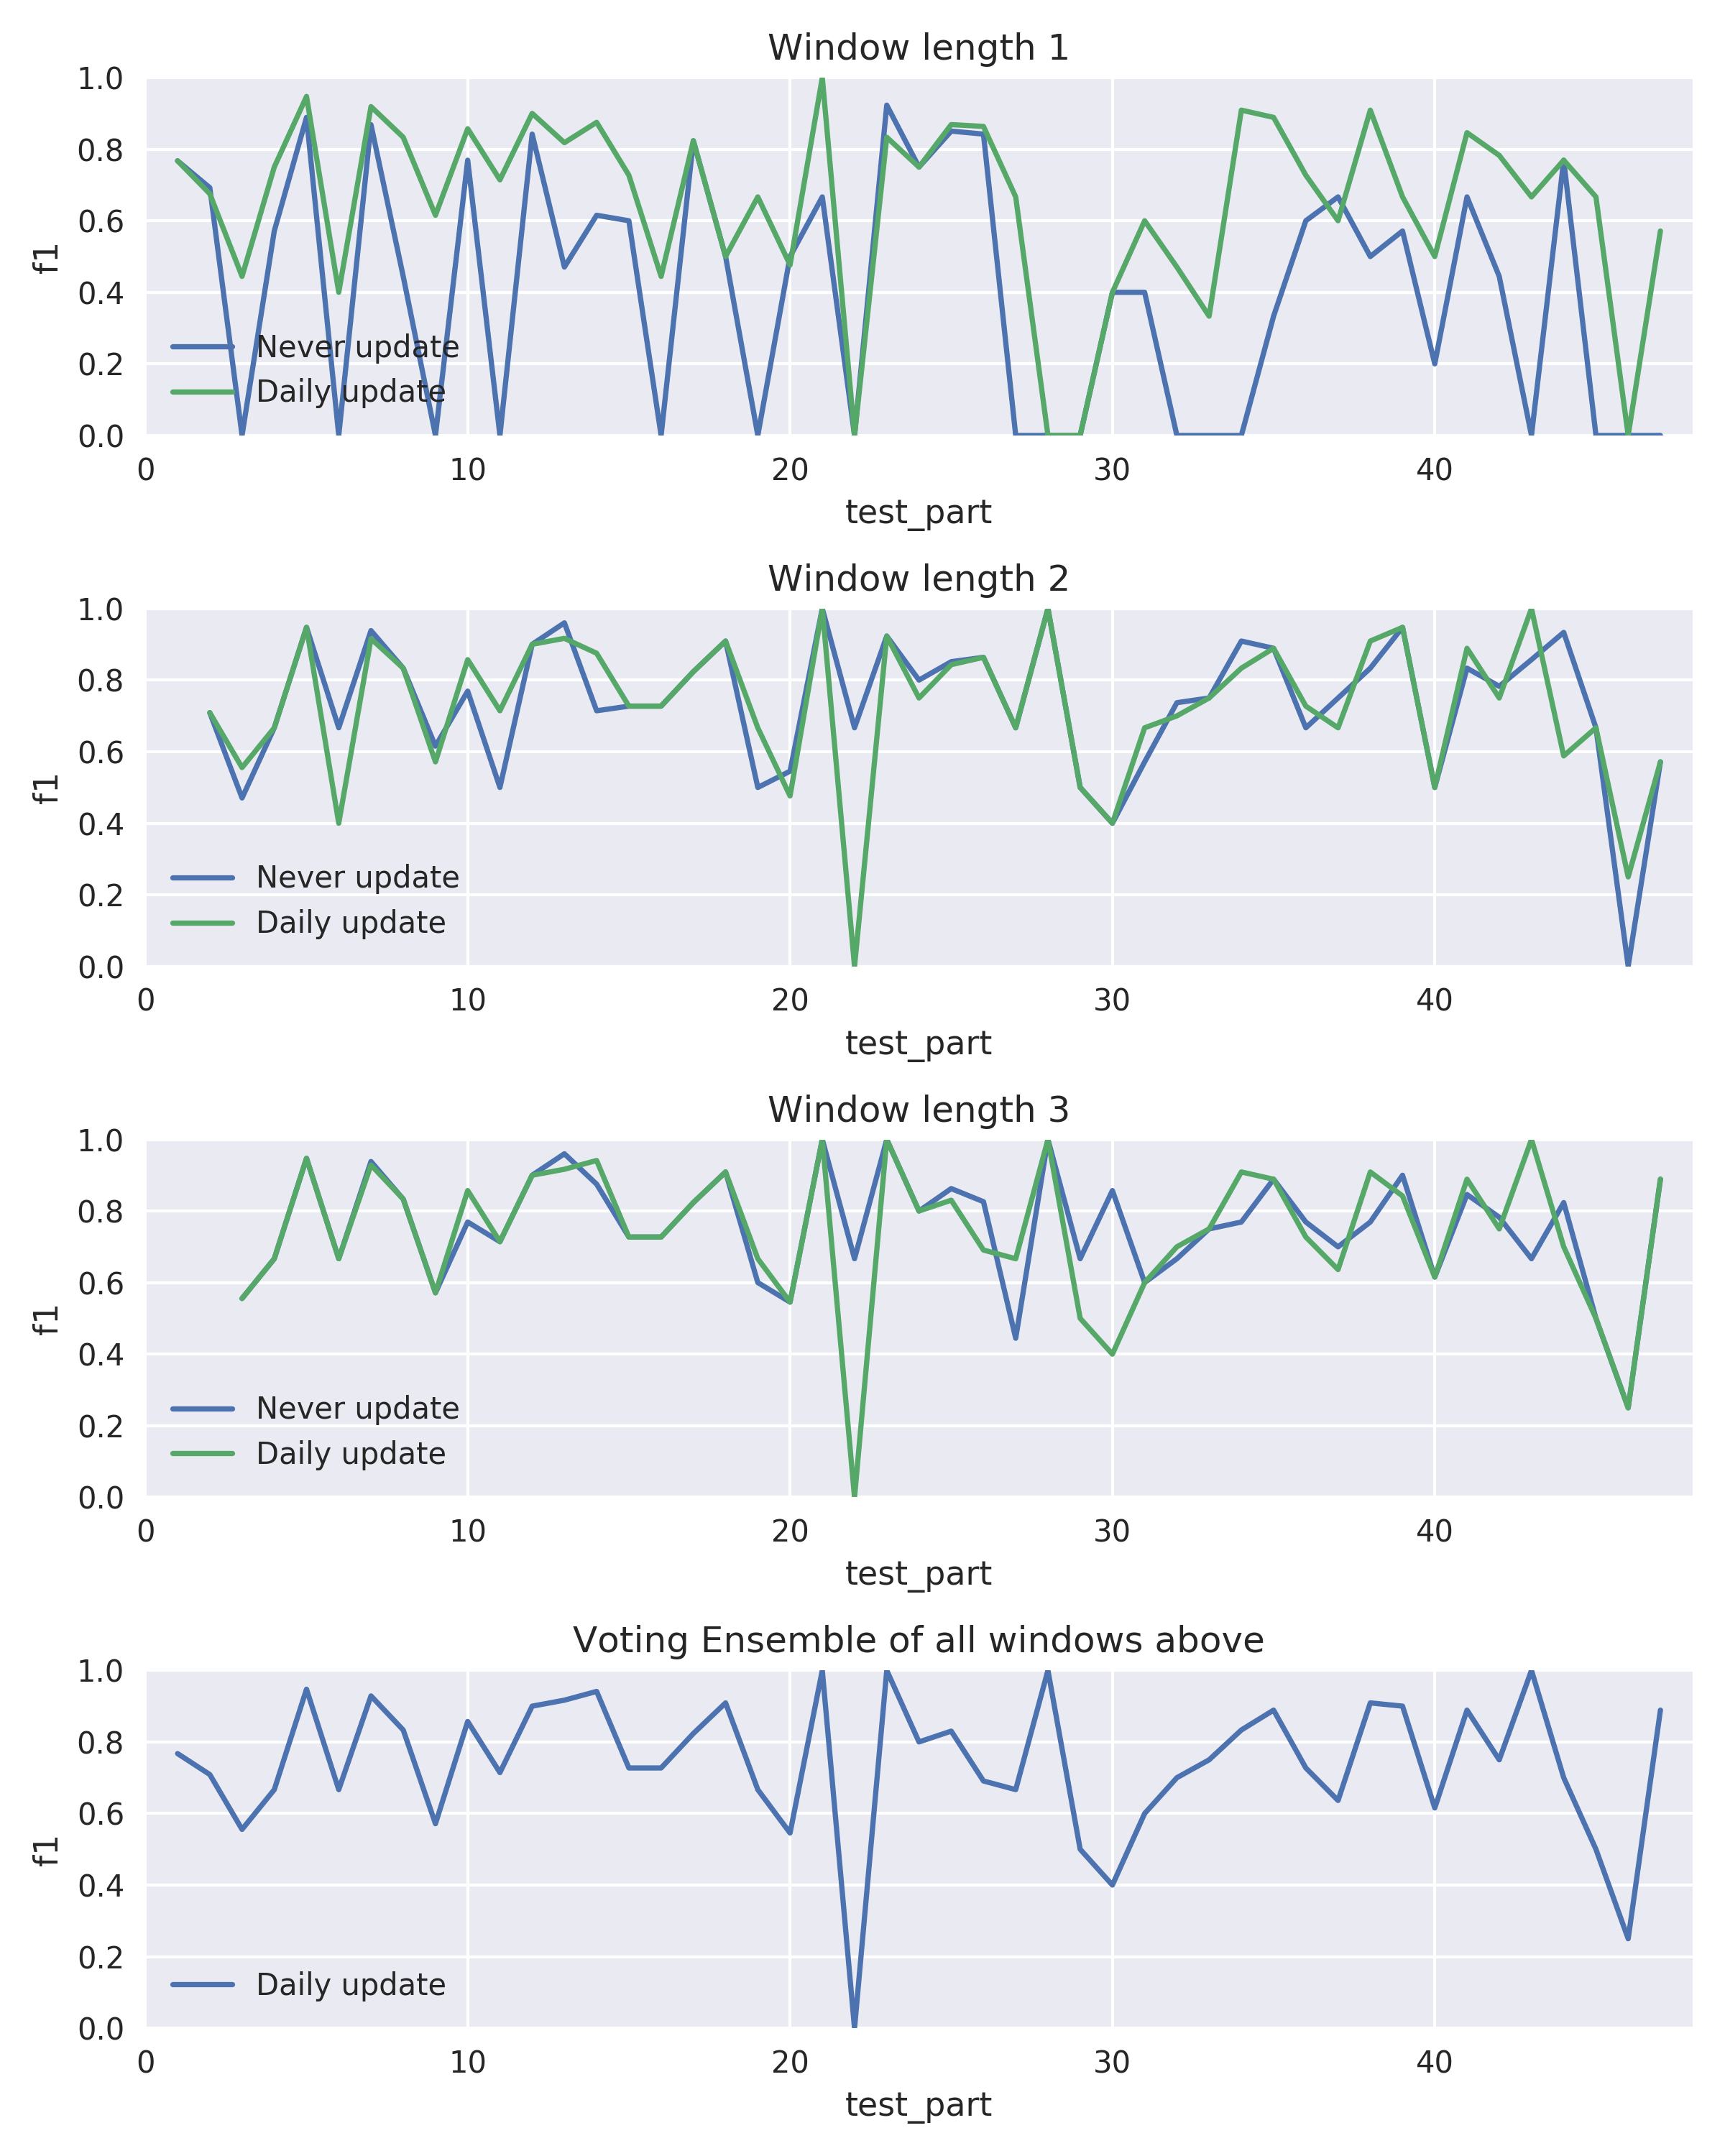
\includegraphics[width=\textwidth]{Images/ensemble.png}
\caption{Accuracy of our Fraud Detection Pipeline}
\label{img:fdp_summary}
\end{figure}


%\centering
%\caption{$F_1$ results of the Fraud Detection Pipeline}
%\label{tbl:fdp_summary}

% Please add the following required packages to your document preamble:
% \usepackage{multirow}
\begin{table}[]
\centering
\footnotesize
\caption{$F_1$ results of the Fraud Detection Pipeline}
\label{tbl:fdp_summary}
\begin{tabular}{|c|c|c|c|c|c|c|}
\hline
\multirow{2}{*}{Window length} & \multicolumn{2}{c|}{Update mechanism}                                    & \multicolumn{2}{c|}{Training $F_1$} & \multicolumn{2}{c|}{Testing $F_1$} \\ \cline{2-7} 
                               & Strategy     & \begin{tabular}[c]{@{}c@{}}Time frame\\ (on testing set)\end{tabular} & Average           & Std             & Average              & Std         \\ \hline
\multirow{2}{*}{1}             & Never update & 0                                                         & 0.4758            & 0.3480          & 0.3331               & 0.3242      \\ \cline{2-7} 
                               & Daily update & 24                                                        & 0.6951            & 0.2312          & \textbf{0.6024}      & 0.2808      \\ \hline
\multirow{2}{*}{2}             & Never update & 0                                                         & 0.7506            & 0.1632          & 0.72                 & 0.2192      \\ \cline{2-7} 
                               & Daily update & 24                                                        & 0.7325            & 0.2304          & \textbf{0.722}       & 0.1893      \\ \hline
\multirow{2}{*}{3}             & Never update & 0                                                         & 0.7808            & 0.1511          & \textbf{0.7351}      & 0.1665      \\ \cline{2-7} 
                               & Daily update & 24                                                        & 0.7571            & 0.2267          & 0.7268               & 0.1871      \\ \hline
Ensemble                & Daily update & 72                                                        & 0.7554            & 0.2164          & \textbf{0.7261}      & 0.1865      \\ \hline
\end{tabular}
\end{table}


\section{Conclusion and other works}

In this survey, we have discussed about several challenges in building an effective Fraud Detection System and then proposed one most suitable and also easy-to-use approach to build our Fraud Detection Pipeline. From the $F_1$ score in the results, it shows that our pipeline could handle the fraud detection problem effectively only with the simplified approach. We also suggest for the readers many things to do to upgrade our pipeline, and it leads to three independent works below:

\begin{itemize}
\item Concept Drift: we have assumed that we could update all of the models in our system every day; in case the data is very huge and the update process takes more than one day to complete then it is a costly task for our system. In chapter 4, we propose a method to decide which model needs to update with the most up-to-date data and we call it as Update Point Estimation algorithm,
\item Imbalance problem: in our proposed pipeline, we used undersampling technique and ensemble learning to handle the imbalance problem (see figure \ref{img:single_rf}) in the credit card dataset which is not only huge but also imbalanced extremely. In chapter 5, we show that why this combination is a most suitable in our case,
\item Algorithms: we only use the Random Forest algorithm in our pipeline, in the rich of literature in fraud detection problem almost algorithms, e.g. supervised learning and unsupervised learning, are used. To the best of our knowledge, a graph-based semi-supervised learning techniques have not been applied to this problem. Therefore in chapter 6, we propose to use an un-normalized graph p-Laplacian based semi-supervised learning combined with the undersampling technique to the fraud detection problem.
\end{itemize}

